\documentclass{beamer}

\usepackage{mathtools,amssymb,mathpartir}
\usepackage[llbracket,rrbracket]{stmaryrd}
\usepackage{tikz}
\usepackage{booktabs}
\usepackage{listings}

\newcommand{\tikznode}[2]{\tikz[remember picture,baseline=(#1.base),inner sep=0pt] \node (#1) {#2};}

\newcommand{\lock}{\text{\tikz[baseline]{
      \fill[rounded corners=.1ex] (-.75ex,0) rectangle (.75ex,1ex);
      \draw[line width=.3ex] (-.4ex,.5ex) -- ++(0,.75ex) arc (180:0:.4ex) -- ++(0,-.75ex);
}}}

\DeclareMathOperator\unbox{unbox}

\title{A Parametric Fitch-style \\ Modal Lambda Calculus}
\author{Axel Forsman}
\institute[CTH]{Chalmers University of Technology}
\date{June 15, 2023}

\begin{document}

\frame{\titlepage}

\begin{frame}{Example: Monads}
  \begin{columns}
    \begin{column}{.49\textwidth}
      \begin{itemize}
      \item Restricts how to get a value out of the box
      \item Used to model e.g. effectful computations
      \end{itemize}
    \end{column}

    \begin{column}{.49\textwidth}
        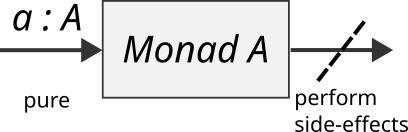
\includegraphics[width=\textwidth]{monad}
    \end{column}
  \end{columns}
\end{frame}

\begin{frame}{Example: S4 modality for run-time codegen}
  \begin{columns}
    \begin{column}{.49\textwidth}
      \begin{itemize}
      \item $\Box A$ models uninterpreted code
      \item Davies, R., \& Pfenning, F. (2001). A modal analysis of staged computation.
      \item Rule of ``necessitation'':

        If $a : A$ is a closed expression, then can get $\Box A$
      \end{itemize}
    \end{column}

    \begin{column}{.49\textwidth}
        
\includegraphics[width=\textwidth]{s4-staged-computation}
    \end{column}
  \end{columns}
\end{frame}

\begin{frame}{Modal axioms that make S4}
  \begin{columns}
    \begin{column}{.49\textwidth}
      \begin{itemize}
      \item Rule of necessitation:

        If have $a : A$ at top-level, then $\Box A$
      \item Axiom K
        $$ \Box (A \to B) \to \Box A \to \Box B $$
      \item Axiom T
        $$ \Box A \to A $$
      \item Axiom 4
        $$ \Box A \to \Box\Box A $$
      \end{itemize}
    \end{column}

    \begin{column}{.49\textwidth}
      \begin{tabular}{@{}lccc@{}} \toprule
        Calculus & Axiom K & T & 4 \\ \midrule
        K & \checkmark & & \\
        T & \checkmark & \checkmark & \\
        K4 & \checkmark & & \checkmark \\
        S4 & \checkmark & \checkmark & \checkmark \\ \bottomrule
      \end{tabular}
    \end{column}
  \end{columns}
\end{frame}

\begin{frame}{Modal operators}
  \begin{equation*}
    \inferrule[$\lambda_\text{K}$/\Box-Intro]{\Gamma, \lock \vdash t : A}{\Gamma \vdash \operatorname{box} t : \Box A} \hspace{4em}
    \pause
    \inferrule[$\lambda_\text{K}$/\Box-Elim]{\Gamma \vdash t : \Box A}{\Gamma, \lock, \Gamma' \vdash \unbox t : A} \mathrlap{\; \lock \notin \Gamma'}
  \end{equation*}
\end{frame}

\begin{frame}{Axiom K with modal operators}
  If
  \begin{equation*}
    \begin{split}
      f &: \Box (A \to B) \\
      x &: \Box A
    \end{split}
  \end{equation*}
  then
  $$ \operatorname{box} \; ((\operatorname{unbox} f) \; (\operatorname{unbox} x)) : \Box B $$
\end{frame}

%% \begin{frame}[fragile]{Example of staged computation}
%%   \begin{lstlisting}[mathescape=true,morekeywords={if,then,else,box,unbox},columns=flexible]
%% mult : $\mathbb N \to \Box (\mathbb N \to \mathbb N)$
%% mult = $\lambda$n : $\mathbb N$. if n = 0
%%     then box ($\lambda$m. 0)
%%     else box ($\lambda$m. m + unbox (mult (n - 1)) m)

%% mult 2 $\mapsto^*$ box ($\lambda$x. x + ($\lambda$y. y + ($\lambda$z. 0) y) x)
%%        = box ($\lambda$x. x + x + 0)
%%   \end{lstlisting}
%% \end{frame}

\begin{frame}{Prior work}
  \begin{figure}
    \centering
    \begin{align*}
      &\inferrule[$\lambda_\text{K}$/\Box-Elim]
      {\Gamma \vdash t : \Box A}
      {\Gamma, \lock, \Gamma' \vdash \unbox_{\lambda_\text{K}} t : A}
      \; \lock \notin \Gamma' &
      &\inferrule[$\lambda_\text{T}$/\Box-Elim]
         {\Gamma \vdash t : \Box A}
         {\Gamma, \Gamma' \vdash \unbox_{\lambda_\text{T}} t : A}
         \; \#_{\lock} (\Gamma') \le 1 \\
         & \inferrule[$\lambda_\text{K4}$/\Box-Elim]
            {\Gamma \vdash t : \Box A}
            {\Gamma, \lock, \Gamma' \vdash \unbox_{\lambda_\text{K4}} t : A} &
            & \inferrule[$\lambda_\text{S4}$/\Box-Elim]
            {\Gamma \vdash t : \Box A}
            {\Gamma, \Gamma' \vdash \unbox_{\lambda_\text{S4}} t : A}
    \end{align*}
    \caption{$\operatorname{unbox}$ rules from
      Clouston, R. (2018). Fitch-style modal lambda calculi.}
  \end{figure}

  Normalization has been given by
  Valliappan, N., Ruch, F., \& Tomé Cortiñas, C. (2022). Normalization for fitch-style modal calculi.
\end{frame}

\begin{frame}{Key idea: Parametric $\unbox$ rule}
  \begin{itemize}
    \item Given a \emph{modal accessibility relation} $\Delta \lhd \Gamma$,
      \begin{equation*}
        \inferrule{\Delta \vdash t : \Box A \\ \Delta \lhd \Gamma}{\Gamma \vdash \operatorname{unbox} t : A}
      \end{equation*}
    \item This gives a \emph{single} parametric calculus
  \end{itemize}
\end{frame}

\begin{frame}{Substitutions}
  $$ \textit{subst} : (\sigma : \operatorname{Sub} \, \Gamma \; \Delta) \to \Gamma \vdash A \to \Delta \vdash A $$

  \begin{equation*}
    \inferrule{ }{\cdot : \operatorname{Sub} \cdot \; \Delta} \qquad
    \inferrule{\sigma : \operatorname{Sub} \Gamma \; \Delta \\ t : \Delta \vdash A}
              {\sigma, t : \operatorname{Sub} \; (\Gamma, A) \; \Delta}
  \end{equation*}
\end{frame}

\begin{frame}{Unified substitutions and modal transformations}
  Used to describe the effect of unboxing.
  \begin{equation*}
    \inferrule{\sigma : \operatorname{Sub} \Gamma \; \Delta \\ \Delta \lhd \Delta'}
              {\operatorname{lock} \sigma \; m : \operatorname{Sub} \; (\Gamma, \lock) \; \Delta'}
  \end{equation*}
\end{frame}

\begin{frame}[fragile]{Implementing \textit{subst}}
  \begin{align*}
    &\cdots \\
    &\textit{subst} \; &&\sigma \; &&(\operatorname{box} t) &&\coloneqq \operatorname{box} \; (\textit{subst} \; (\operatorname{lock} \sigma \; \tikznode{lhd1}{$\lhd_\lock$}) \; t) \\
    &\textit{subst} \; &&\sigma \; &&(\operatorname{unbox} t \; m) &&\coloneqq \operatorname{unbox} \; (\textit{subst} \; \sigma' \; t) \; m' \\
    &\mathrlap{\quad \text{where } m', \sigma' = \textit{rewind} \; m \; \sigma}
  \end{align*}
  \tikz[remember picture,overlay]{
    \draw (lhd1.north) -- ++(.5cm,1cm) node[anchor=south] {$\lhd_\lock : \Gamma \lhd \Gamma, \lock$};
  }
  \pause
  \begin{center}
    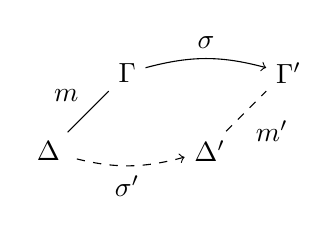
\begin{tikzpicture}
      \node (Γ) at (1,1) {$\Gamma$};
      \node (Γ') at (3,1) {$\Gamma\mathrlap'$};
      \node (Δ) at (0,0) {$\Delta$};
      \node (Δ') at (2,0) {$\Delta\mathrlap'$};
      \path (Γ) edge[->,bend left=15] node[above] {$\sigma$} (Γ')
      edge[-] node[auto=right] {$m$} (Δ)
      (Δ') edge[-,dashed] node[auto=right] {$m'$} (Γ')
      edge[<-,dashed,bend left=15] node[below] {$\sigma'$} (Δ);
    \end{tikzpicture}
  \end{center}
\end{frame}

\begin{frame}{Equational theory}
  \begin{align*}
    \llap{$\beta$ equivalence:}& \quad
    \inferrule{\Delta, \lock \vdash t : A \\ m : \Delta \lhd \Gamma}{\unbox \; (\operatorname{box} t) \; m \sim \textit{subst} \; (\operatorname{lock} \textit{id}_s \; m) \; t} \\
    \llap{$\eta$ equivalence:}& \quad
    \inferrule{\Gamma \vdash t : \Box A}{t \sim \operatorname{box} \; (\operatorname{unbox} t \; \lhd_\lock)}
  \end{align*}
\end{frame}

\begin{frame}{Normalization by Evaluation}
  $$ nf : \Gamma \vdash A \to \text{Nf} \; \Gamma \; A $$

  \begin{gather*}
    \inferrule{x : \text{Ne} \; \Gamma \; \iota}{\operatorname{ne} x : \text{Nf} \; \Gamma \; \iota} \quad
    \cdots\quad
    \inferrule{x : \text{Nf} \; (\Gamma, \lock) \; A}{\operatorname{box} x : \text{Nf} \; \Gamma \; (\Box A)}
  \end{gather*}
  \pause
  \begin{gather*}
    \inferrule{x : A \in \Gamma}{\operatorname{var} x : \text{Ne} \; \Gamma \; A} \quad
    \cdots\quad
    \inferrule{x : \text{Ne} \; \Delta \; (\Box A) \\ m : \Delta\lhd\Gamma}{\operatorname{unbox} x \; m : \text{Ne} \; \Gamma \; A}
  \end{gather*}
\end{frame}

\begin{frame}{Semantic values}
  \begin{equation*}
    \begin{split}
      \llbracket \iota \rrbracket_\Gamma &\coloneqq \text{Nf} \; \Gamma \; \iota \\
      \llbracket A \to B \rrbracket_\Gamma &\coloneqq \forall \Delta. \, \Gamma \subseteq \Delta \to \llbracket A \rrbracket_\Delta \to \llbracket B \rrbracket_\Delta \\
      \llbracket \Box A \rrbracket_\Gamma &\coloneqq \forall \Gamma', \Delta. \, \Gamma \subseteq \Gamma' \to \Gamma'\lhd\Delta \to \llbracket A \rrbracket_\Delta
    \end{split}
  \end{equation*}

  Environments $\gamma : \operatorname{Env} \Gamma \; \Delta$
\end{frame}

\begin{frame}
  \begin{align*}
    &\mathrlap{\text{Evaluation} \quad \llbracket-\rrbracket : \Gamma \vdash A \to \forall\Delta.\, \operatorname{Env} \Gamma \; \Delta \to \llbracket A \rrbracket_\Delta} &&\\
    &\llbracket x \rrbracket \; \gamma &&\coloneqq \text{lookup } x \text{ in } \gamma \\
    &\llbracket \operatorname{box} t \rrbracket \; \gamma &&\coloneqq \lambda w \; m.\, \llbracket t \rrbracket \; (\operatorname{lock} \; (\operatorname{wk}_e w \; \gamma) \; m) \\
    &\llbracket \operatorname{unbox} t \; m \rrbracket \; \gamma &&\coloneqq \llbracket t \rrbracket \; \gamma' \; \textit{id}_\subseteq \; m' \quad \text{where } m' , \gamma' = \textit{rewind} \; m \; \gamma \\
    &\mathrlap{\text{Reification} \quad \downarrow^A : \llbracket A \rrbracket_\Gamma \to \operatorname{Nf} \; \Gamma \; A} &&\\
    &\downarrow^{\Box A} a &&\coloneqq \operatorname{box} \; (\downarrow^A (a \; \textit{id}_\subseteq \; \lhd_\lock)) \\
    &\mathrlap{\text{Reflection} \quad \uparrow^A : \operatorname{Ne} \; \Gamma \; A \to \llbracket A \rrbracket_\Gamma} &&\\
    &\uparrow^{\Box A} x &&\coloneqq \lambda w \; m.\, \uparrow^B (\operatorname{unbox} \; (\operatorname{wk}_{\operatorname{Ne}} w \; x) \; m)
  \end{align*}

  $$ nf \; t \coloneqq\, \downarrow (\llbracket t \rrbracket \; \textit{freshEnv}) $$
\end{frame}

\begin{frame}{Calculus parameters for proving correctness}
  \begin{itemize}
  \item Rewinding $\operatorname{lock} \sigma \; m$
    with a modal accessibility relation $\Gamma \lhd \Gamma, \lock$
    should work as expected, i.e.\@ give back $m$ and $\sigma$.
  \item The operation $\textit{rewind}$ should distribute over composition.
  \item $\textit{rewind}$ should preserve identity.
  \item $\textit{rewind}$ should commute with weakening and substitution composition.
  \end{itemize}
\end{frame}

\begin{frame}{Instantiations}
  \begin{itemize}
  \item Calculus K:
    \begin{align*}
      \Delta \lhd_\text{K} \Gamma &\coloneqq \exists\Xi.\, \lock\notin\Xi \;\text{and}\; (\Gamma = \Delta, \lock, \Xi)
      \intertext{\item Calculus S4:}
      \Delta \lhd_\text{S4} \Gamma &\coloneqq (\Gamma = \Delta) \;\text{or}\; (\exists\Xi.\, \Gamma = \Delta, \lock, \Xi)
    \end{align*}
  \end{itemize}
\end{frame}

\begin{frame}{Future work}
  \begin{itemize}
  \item Extend with more language extensions
  \item Generalize to include other modal axioms, such as axiom R ($A \to \Box A$)
  \end{itemize}
\end{frame}

\end{document}
